\section{Introduction}
\label{sec:intro}

Graphs are a ubiquitous model to represent objects and their complex relations,
including protein interaction networks and genomic graphs in biology \cite{RHS13},
chemical compounds \cite{WMFP05}, call graphs in program flow analysis \cite{control},
social networks \cite{Kempe}, and government and medical records \cite{SH12}.
Efficient mining of hidden patterns play an important role in developing data-driven
methodologies for analyzing graphs
resulting from such datasets.
Research on graph mining has emerged as one of the hottest topics in recent years due to its wide applications in a variety of fields including
drug discovery \cite{KK01,NK05,YH02}, molecular activity prediction \cite{JinYW10,TCG09},
predicting disease susceptibility from gene expression data \cite{RHS13,DI11}, clustering and classification of graphs \cite{DKWK05,YCHY08}, and anomaly detection \cite{ATK15}.
Several variants of graph pattern mining have been proposed,
such as frequent subgraphs \cite{YH02,EASK14}, approximate subgraphs \cite{KYW10}, discriminant and statistically significant subgraphs \cite{TCG09,RS09,YCHY08}, representative subgraphs \cite{CHSBZ08,ZYL09}, etc.
%--- their scalable algorithms
%were implemented; besides, they were extensively surveyed and compared, e.g., in \cite{HCXY07,WMFP05,AW10,KR17}.
%
\begin{figure}[t!]
\vspace{-2mm}
\centering
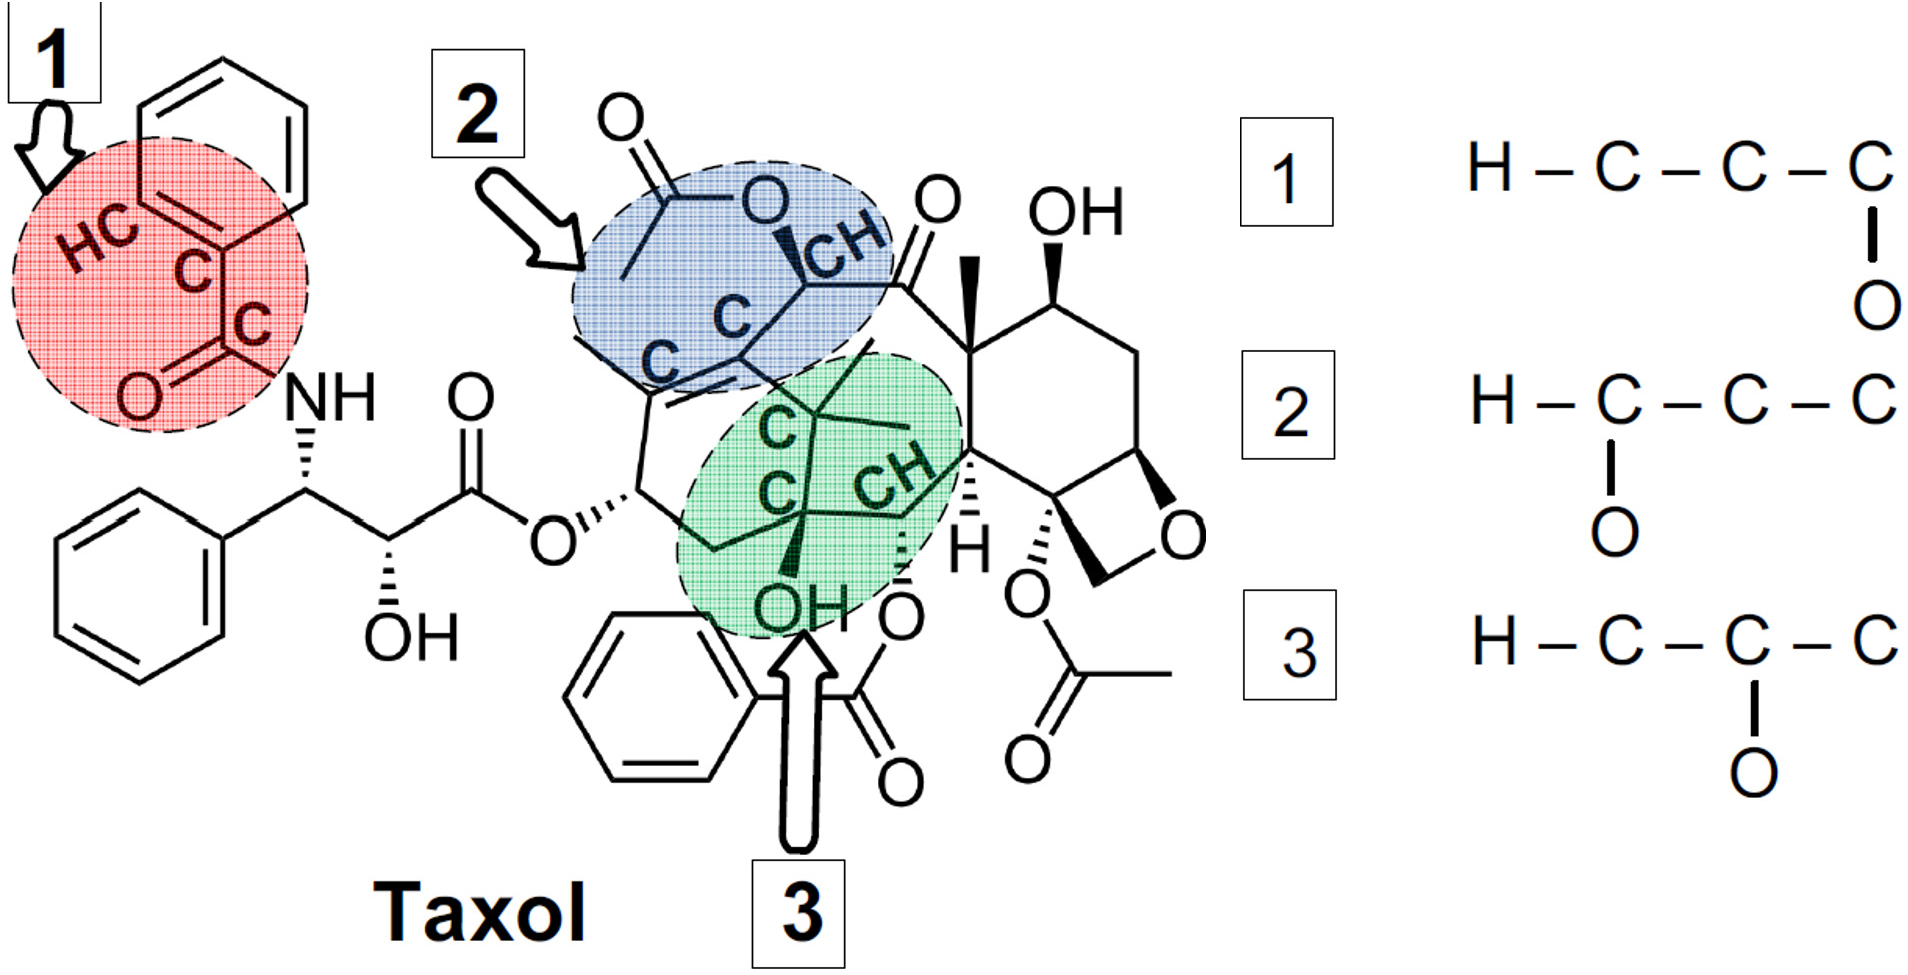
\includegraphics[width=2.2in]{images/taxol.pdf}
\caption{Correlation between {\sf CCCH} and {\sf O} in {\sf Taxol}, an anti-cancer drug. {\sf CCCH} and {\sf O}
occur closely for several times, but they are connected in different ways.}
\label{fig:taxol}
\vspace{-0.10in}
\end{figure}
%


In spite of tremendous progress being made in the area of graph pattern mining, surprisingly the problem of exploring correlations between subgraphs
in a single, large graph has not been investigated in the past. In particular, we define a pair of subgraphs as correlated if
they co-occur frequently in proximity within a single graph. Correlated subgraphs are different from frequent subgraphs due to
the flexibility in which the constituent subgraphs can be connected within different instances of a correlated pattern. To elaborate, in Figure~\ref{fig:taxol},
we highlight three regions inside the structure of the chemical compound {\sf Taxol}, an anti-cancer drug, where {\sf CCCH} and {\sf O} occur closely,
albeit they are connected in different ways in all three instances. For simplicity, we do not consider the edge types (i.e., single- vs. double-bond)
in this example. This figure illustrates that while {\sf CCCH} and {\sf O} form a correlated subgraph pair, the individual instances, e.g., {\sf HCC(-O)C}
may not be frequent; and hence, existing frequent subgraphs mining techniques would not discover such corrected patterns.

\vspace{-0.05in}
\subsection{Applications}
The problem of detecting correlated subgraphs from a single, large graph arises in many real-world scenarios, including biological,
social, chemical, and ecological networks. We discuss two concrete examples below.

\begin{figure}
 \vspace{-0.20in}
 \centering
	\begin{subfigure}[t]{0.21\textwidth}
		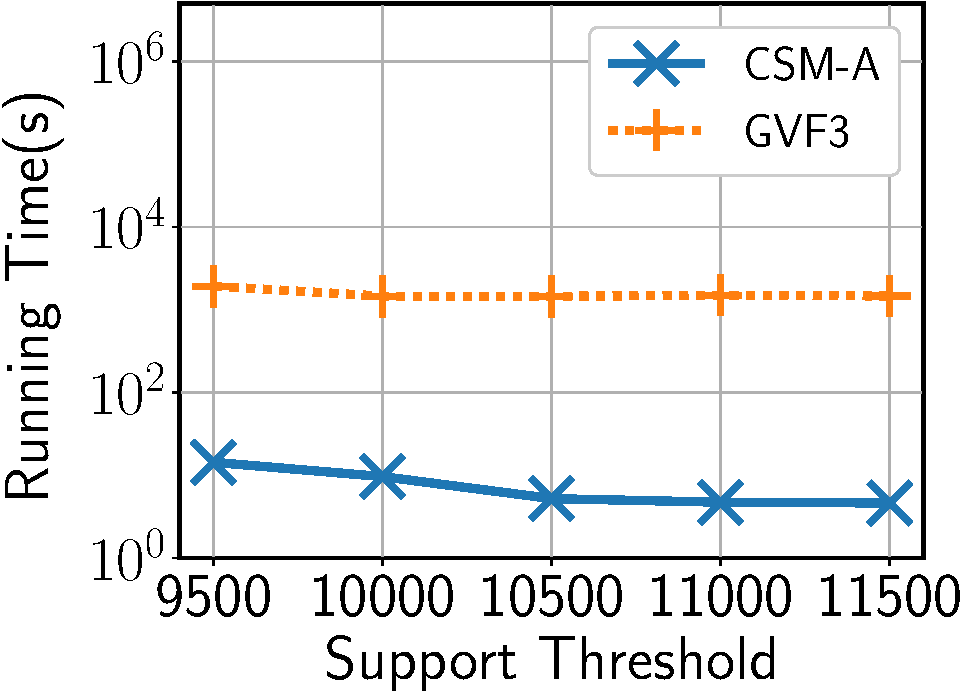
\includegraphics[scale=0.24]{img2/mico/mico_gvf3.pdf}
		\caption{\scriptsize $Mico$ dataset (small)}
		\label{fig:intro_micogvf3}
    \end{subfigure}%
    \hspace*{\fill}
	\begin{subfigure}[t]{0.23\textwidth}
		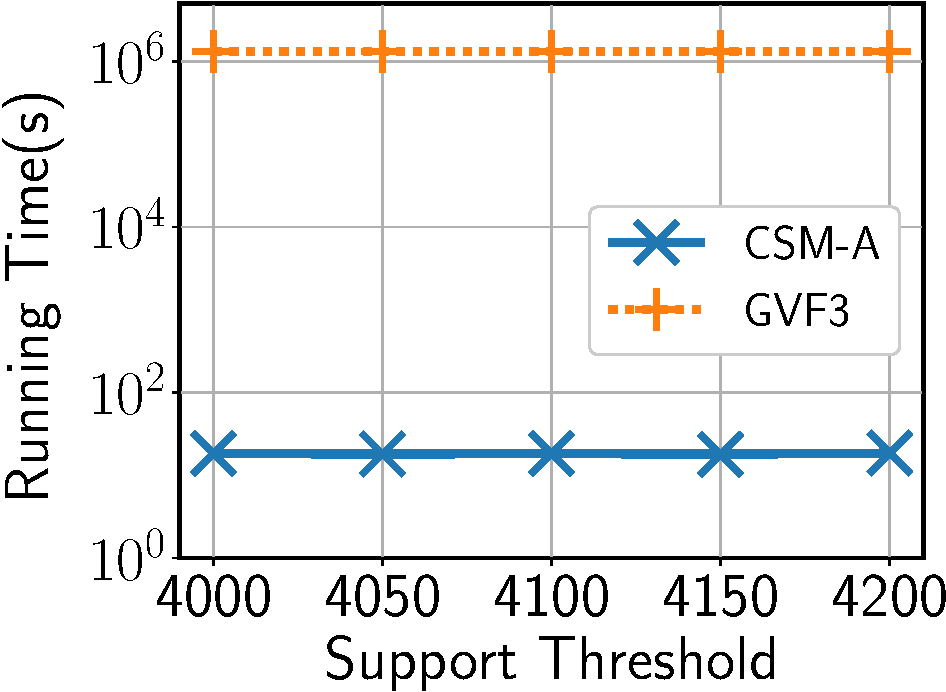
\includegraphics[scale=0.24]{img2/citationdblp/citationdblp_gvf3.pdf}
		\caption{\scriptsize $DBLP\ Citation$ dataset (large)}
		\label{fig:intro_citationdblpgvf3}
	\end{subfigure}%
	\caption{Our performance against GraMi+VF3 baseline}
	\label{fig:motivation}
	\vspace{-0.1in}
\end{figure}

\spara{$\bullet$ Co-operative functions in biological networks.} In genome graph of an individual, a node represents a gene,
and each edge denotes the interaction between two genes. In practice, there are some combinations of dominant genes that
occur frequently, and they are more likely to express critical phenotypes of the individual.
Past studies have shown that some pairs of dominant gene combinations co-occur with each other in each individual,
and such co-occurring patterns reflect the joint functionality that are needed for co-operative biological functions such as chemical bonds
and binding sites \cite{LFSW14}. Based on pairs of correlated genes, we can predict co-operative biological functions of an
individual. Besides, the absence of such correlations indicates anomalies and diseases.
Analogously, in a protein interaction network, correlated frequent subgraphs represent recurring functional units,
identification of which could assist in predicting new protein functionalities.

%\vspace{-0.05in}
\spara{$\bullet$ Co-occurrence patterns in ecological networks.}
In ecology, co-occurrence patterns are used to explore interactions between organisms
and environmental effects on co-existence within biological communities \cite{WHH14}.
Exploration of inter-taxa relationships can help identify potential biotic interactions, habitat affinities, and shared physoilogies,
that could guide more focused studies and experiments. For example, Barberan et al. \cite{BBCF12} analyzed
over $160\,000$ bacterial and archaeal $16S$ rRNA gene sequences from $151$ soil samples, collected
from a wide variety of ecosystem types, in order to demonstrate the utility of network
analyses and for evaluating whether soil microorganisms tend to co-occur more
than expected by chance, and how these
ecological categories shape network structure of inter-taxa and extra-taxa relationships.
These tasks can be achieved by mining correlated subgraphs in a single large graph
representing the soil microbial community.

\vspace{-0.05in}
\subsection{Technical Challenges and Baselines}
\label{sec:baseline}
%The problem that we study is a non-trivial one.
%
%\squishlist
\textbf{Frequent subgraphs mining. } Detecting correlated subgraphs is more difficult
than the frequent subgraphs mining problem \cite{WMFP05}, which already has an exponential search space, that is, a graph with $m$ edges
can have $2^m$ subgraphs. For correlated subgraphs mining, the search space is doubly-exponential, because
one needs to compute the correlation between every pair of subgraph instances.
 Additionally, unlike frequent subgraphs mining,
correlated subgraphs mining is neither downward-closure, nor upward-closure (we shall demonstrate this formally
in \S~\ref{sec:problem}), thereby making it difficult to directly apply apriori-based pruning techniques.

 Last, but not least, only finding the frequent subgraphs is not sufficient for our problem. Since we call subgraph $A$ to be correlated to $B$ if their \emph{instances} are frequently located close to each other, we need to enumerate \emph{all} instances of those frequent subgraphs for computing the correlation
between pairs. This makes our problem more challenging both from computation and memory perspective. To establish this point empirically, we perform frequent subgraphs mining using GraMi~\cite{EASK14}, and for each frequent subgraph, we enumerate all of its instances using the state-of-the-art VF3 algorithm~\cite{CarlettiFSV18} and finally compute the correlated pairs. Fig.~\ref{fig:motivation} presents the result on two datasets; the dataset description is provided in Table~\ref{ref:datasets}. We observe that the frequent subgraphs mining based approach takes more than $15$ days in the DBLP-Citation network dataset. On the other hand, the proposed approach, CSM, is up to $5$ orders of magnitude faster. Real networks contain millions of nodes and it is desirable to obtain results within minutes. In this paper, we achieve this task with a single-step correlated subgraphs mining algorithm. %As visible in Fig.~\ref{fig:motivation}, the proposed approach, denoted as CSM, is XXX orders of magnitude faster.


\textbf{Correlated subgraphs mining in graph databases. } The closest work to ours in the space of correlated subgraphs mining is by Ye et al.\cite{KCY09}. However, there are three fundamental differences. First, Ye et al. target the graph database scenario where there are multiple graphs and the frequency of a subgraph is defined as the number of database graphs containing the given subgraph. In our problem, we target the single large graph scenario where the frequency of a subgraph is the number instances within the single large graph. It is well known from the frequent subgraphs mining literature \cite{EASK14,KhanR17}, that the single-large-graph scenario imposes a more severe scalability challenge since subgraph enumeration is more expensive. Second, the definition of correlated patterns is different. More specifically, in \cite{KCY09}, two subgraphs $A$ and $B$ are correlated if the containment of $A$ within a data graph increases the likelihood of containing $B$ as well. In our problem, two subgraphs $A$ and $B$ are correlated if the instances of $A$ are frequently located in \emph{close proximity} to the instances of $B$. Third, we have the concept of proximity in our problem, which is absent in \cite{KCY09}. Owing to these fundamental differences in the formulation, the resulting algorithmic challenges are different as well.

%We next describe why state-of-the-art techniques cannot be trivially adapted to find correlated subgraphs
%in a single, large graph.
%
%\spara{$\bullet$ Difficulties with Frequent Subgraphs Enumeration.}
%One can apply state-of-the-art frequent subgraphs mining techniques over a single graph (e.g., {\sf GRAMI} \cite{EASK14})
%to first identify all frequent subgraphs, compute correlations between every pair, and then report the
%highly correlated ones. However, this approach has several limitations.
%{\bf (1)} Many existing frequent subgraphs mining algorithms including {\sf GRAMI}
%report only the frequent subgraphs, and not their instances in the large graph.
%Thus, we separately need to enumerate all their instances using a subgraph matching algorithm
%(e.g., {\sf VF2} \cite{CFSV04}, $\textsf{Turbo}_\textsf{ISO}$ \cite{HLL13}, $\textsf{Dual}_\textsf{ISO}$ \cite{SJKFMR14}),
%which is necessary for correlation computation, but is expensive over large graphs (Figure XX).
%{\bf (2)} We are often interested in finding only the top-$k$ correlated pairs. However, the aforementioned
%frequent subgraphs mining and enumeration approach will compute correlations across every frequent subgraphs,
%which is expensive and mostly redundant. This brings the following critical question: {\em Can we mine the (top-$k$) correlated
%subgraphs in one single step}, as opposed to the aforementioned two-step frequent subgraphs mining and enumeration approach?
%The answer to this question, as we shall demonstrate in \S~\ref{sec:algorithms}, is affirmative.
%
%\begin{figure}[t!]
%\vspace{-2mm}
%\centering
%\subfigure[] {
%\includegraphics[scale=0.17]{images/yeast1}
%\label{fig:yeast1}
%}
%\subfigure[]  {
%\includegraphics[scale=0.17]{images/yeast2}
%\label{fig:yeast2}
%}
%\subfigure[]  {
%\includegraphics[scale=0.17]{images/yeast3}
%\label{fig:yeast3}
%}
%\vspace{-2mm}
%\caption{\scriptsize Correlated subgraphs discovered in the {\em Yeast} protein dataset. Nodes are annotated with protein functions (node labels).}
%\label{fig:yeast}
%\vspace{-6mm}
%\end{figure}


%\spara{$\bullet$ Difficulties with Proximity Patterns.} Recently, various approximate-frequent-subgraphs mining techniques have been
%proposed, e.g., proximity patterns \cite{KYW10} that relax the rigid structure constraint of frequent subgraphs. In stead, they identify
%a group of node labels that co-occur frequently in the neighborhood. However, such proximity patterns are often unable to capture
%the semantics of our novel correlated subgraphs. As an example, in Figure~\ref{fig:yeast},
%we present three correlated patterns identified from
%the {\em Yeast} (Saccharomyces cerevisiae) protein dataset \cite{}, where protein functions are used as node labels. These
%correlated patterns indicate that {\em transferase} and {\em hydrolase} activities are associated with {\em ion} binding,
%which is due to the fact that {\em transferase} and {\em hydrolase} undergo motions upon ligand ({\em ion}) binding
%to achieve their functions \cite{KAOK08}. However, {\em transferase} and {\em hydrolase} catalyze different chemical
%reactions and express different dynamic responses upon ligand ({\em ion}) binding. It means that {\em hydrolase} and {\em transferase}
%activities are usually not connected with each other directly and they usually connect to {\em ion} binding \cite{KKO09}.
%This is indeed reflected in our discovered correlated patterns, because there is no direct edge between {\em hydrolase} and {\em transferase}.
%On the other hand, the proximity pattern mining algorithm \cite{KYW10} reports
%$\langle${\em hydrolase}, {\em transferase}, {\em ion binding}$\rangle$ as one
%proximity pattern, thus it is unable to capture the fact that {\em hydrolase} and {\em transferase}
%activities are not connected with each other directly.

\vspace{-0.1in}
\subsection{Contributions and Roadmap}
%In this paper, we design a single-step, best-first exploration algorithm to detect correlated subgraphs,
%coupled with efficient top-$k$ pruning and various optimization techniques.
The main contributions of this paper are as follows:
\squishlist
\item We formulate the problem of \emph{correlated subgraphs mining} in a single large graph, which is defined as a pair of subgraph patterns that frequently
co-occur in proximity within a single graph (\S~\ref{sec:preliminaries}).
\item The key differentiating factor in our problem compared to existing subgraph mining problems is that we not only need to identify the subgraph patterns, but also enumerate and store all of its instances. This requirement imposes a huge scalability challenge on both computation and storage. We tackle this issue by designing a novel data structure called \emph{$\mathcal{R}$eplica}, which stores all instances of a subgraph pattern on demand in compressed manner. %$\mathcal{R}$eplica not only brings down the computation cost, but also reduces the storage cost drastically. 
 Using $\mathcal{R}$eplica as the data storage platform, we design a single-step, best-first exploration algorithm to detect correlated subgraph pairs efficiently (\S 3). We further speed up the mining process by designing a near-optimal approximtion algorithm (\S 4).
\item We empirically demonstrate effectiveness and efficiency of our methods on seven real graphs, while also detailing concrete case studies. We establish that the proposed algorithm is up to $5$ orders of magnitude faster than baseline strategies and scalable in million-sized networks (\S \ref{sec:experiments}).
\squishend
